\chapter{Implementation}
    Application which will all principles describes in~\ref{analysis}. Created project is focused on the design and development of the Automatic prediction model builder system in the form of an application with a user-friendly user interface, which will be implemented in the cloud environment. As a development environment Matlab ecosystem was used.
    \section{Mathematical models}
    Prediction models were based mainly on the principle of linear prediction (LP) and its modifications, such as non-integer linear prediction (fractional linear prediction - FLP), LP extended by parameters capable of capturing short-term and long-term trendiness in data (extended linear prediction - ELP), etc., which will be extended by further statistical methods such as Monte Carlo, Markov chains, etc.\\
    \\
    For the identification of the appropriate structure of economic and behavioral models and the identification of the parameters of the selected models, machine learning algorithms will be used, which will provide the optimal solution for the selected data and thus the use-case.
    \section{Application}
    This application would make it possible to easily and accurately predict various socioeconomic macro and micro indicators, such as gross/net domestic/national product, economic wealth, unemployment, inflation, average/minimum wage, purchasing power of the population but also the behavior of customers (customers can also be perceived as households), intended for sectors such as public or state administration, public planning (but also private) finance, banking.\\
    \\
    From the point of view of commercial use, a possible application would be predicting the number of customers and the number of orders, the company's income, the success of marketing strategies, or on the basis of the prediction, the planning of warehouse stocks.
    \begin{figure}
        \centering
        \begin{subfigure}[b]{0.4\textwidth}
            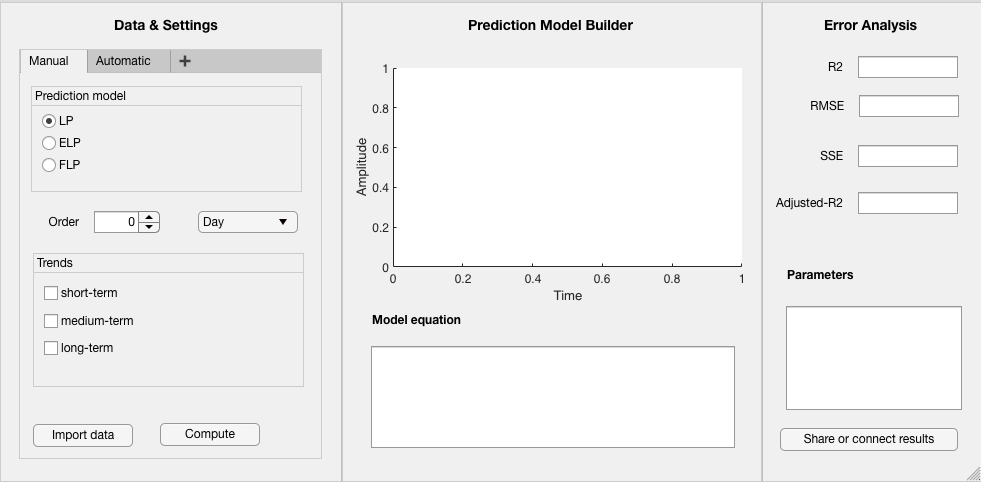
\includegraphics[width=\textwidth]{figures/manual.png}
            \caption{Manual settings}
            \label{fig:manual}
        \end{subfigure}
        \hspace{0.1\textwidth}
        \begin{subfigure}[b]{0.4\textwidth}
            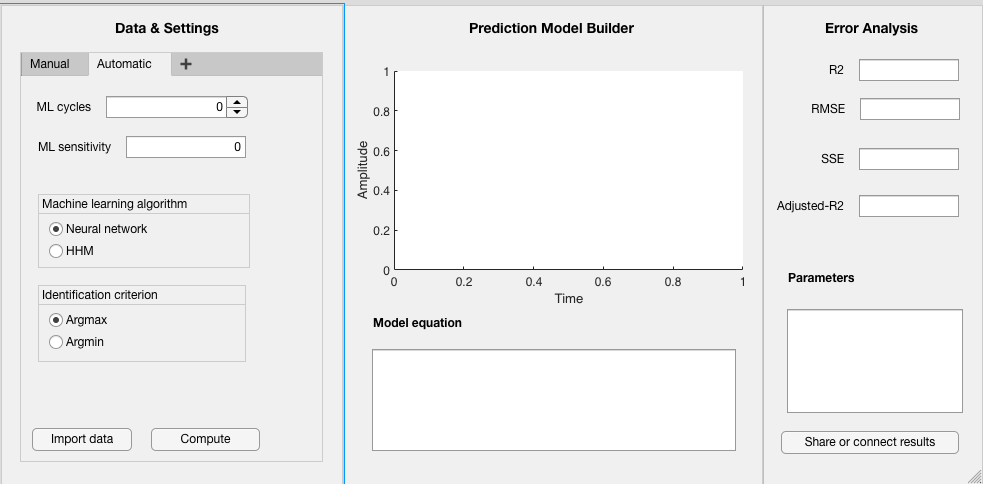
\includegraphics[width=\textwidth]{figures/auto.png}
            \caption{Automatic settings}
            \label{fig:automatic}
        \end{subfigure}
        \begin{subfigure}[b]{0.4\textwidth}
            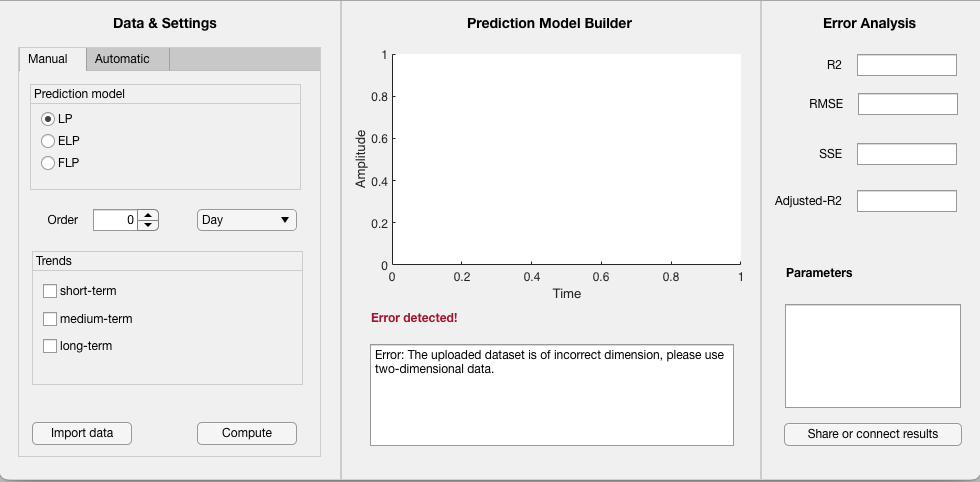
\includegraphics[width=\textwidth]{figures/warning.png}
            \caption{Dataset warning}
            \label{fig:warning}
        \end{subfigure}
        \hspace{0.1\textwidth}
        \begin{subfigure}[b]{0.4\textwidth}
            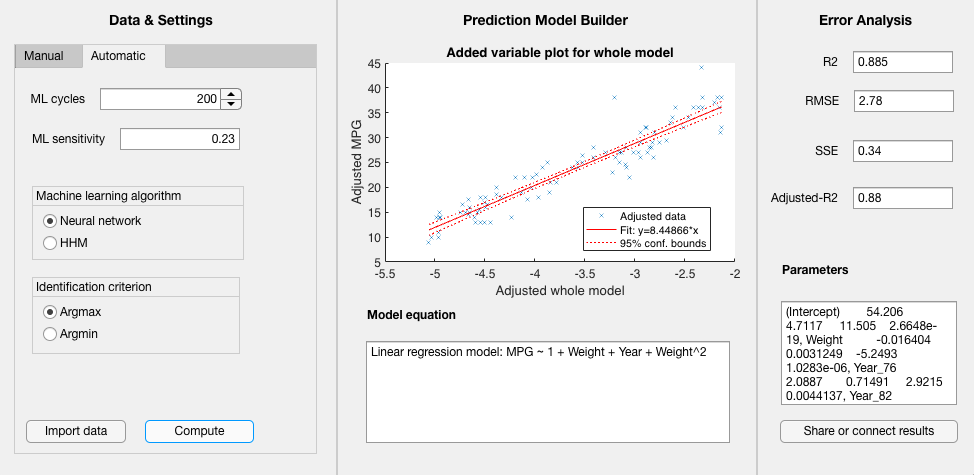
\includegraphics[width=\textwidth]{figures/result.png}
            \caption{Results}
            \label{fig:results}
        \end{subfigure}
        \label{fig:appoverview}
        \caption{Application overview}
    \end{figure}
        \subsection{Import datasets}
        First step to get results from predictive application. Use the button in the left
        bottom corner~\ref{fig:manual} to import our dataset. Application is able to
        process datasets in csv or excel format. Application is trying to identify
        your dataset by the setting~\ref{subsec:setting}. If the problem in our imported
        dataset is detected, application show warning~\ref{fig:warning} with the tips
        how to preparte your dataset in a better way.
        \subsection{Setting}\label{subsec:setting}
        Application has two way of settings, we can define parameters of our model manualy or
        we can choose automatic setting of application to detect the best prediction model
        based on inserted dataset.\\
        \\
        \textbf{Manual setting}\\
        Manual setting is to create a prediction model based on linear prediction. 
        We are able to use these parameters:
        \begin{itemize}
            \item \textbf{Prediction model}\\
            Choose one of type from Linear prediction~\ref{eg:lp}, Extended linear prediction~\ref{eg:elp},
            Fraction linear prediction~\ref{eg:flp}.
            \begin{equation}\label{eg:elp}
                \hat{x}(n) = \left(\sum_{i=1}^{p} a_i x(n-i) + \sum_{i=1}^{q} b_i x(n-S-i)\right) * \gamma(n),
            \end{equation}
            \\
            where $\hat{x}(n)$ is the~predicted value of the~order at time $n$, $x(n-i)$ are the~past short-therm predition part $p$ samples of the~dataset, $x(n-S-i)$ are the~past long-term prediction part with seasonal shift $S$, and $a_i$ and $b_i$ are the~predictors coefficients. The~order of the~predictor is $p$ for short-term and $q$ for the long-term linear prediction. The seasonal weights is represent by $\gamma(n)$.\\
            \\
            \begin{equation}\label{eg:lp}
                \hat{x}(n) = \sum_{i=1}^{p} a_i x(n-i),
                \label{eq:linear-predictor}
            \end{equation}
              
            where $\hat{x}(n)$ is the~predicted value of $x(n)$, $p$ is the~order of the~predictor, and $a_i$ are the~predictor coefficients. The~predictor coefficients can be found by minimizing the~prediction error.
            \\
            \begin{equation}\label{eg:flp}
                \hat{x}(n) = a_1 x(n-i) + a_2 \frac{h^\alpha}{T(1 + \alpha)}D^\alpha x(n-1),
                \label{eq:linear-predictor}
            \end{equation}
            
            that uses two-samples memory, is independent of the order of fractional derivative $\alpha$~\cite{DESPOTOVIC2018158}.
            \item \textbf{Order of predictor}\\
            In this step we are able to set up the order of linear prediction and the
            period of predicted values.
            \item \textbf{Trends detection}\\
            In this setting you are able to choose the length of the period to 
            identify the prediction model parameters and trends.
        \end{itemize}
        \noindent
        \textbf{Automatic setting}\\
        Autoimation setting we can used for set up the parameters of neural network,
        which will be used to set up all optimal parameters for prediction. For set up
        automation part of application we are able to use these parameters:\\
        \begin{itemize}
            \item \textbf{Machine learning cycles}\\
            Number of observations use to find optimal parameters of the model.
            \item \textbf{Machine learning sensitivity}\\
            Sensitivity is a measure of how well a machine learning model can
            detect positive instances. It is also known as the true positive rate
            (TPR) or recall.
            \item \textbf{Machine learning alghoritm}\\
            In this section we are able to choose the neural network or hidden markov model
            to run in backround. HMM is statistical approach and in specific dataset can provide
            beter results.
            \item \textbf{Identification criteria}\\
            In this part we can choose the maximalization or minimalization as a function
            to found optimal parameters.
        \end{itemize}
        \subsection{Results}\label{subsec:result}
        Fo our test purpose we used the automatic setting of the application and try to run
        over our dataset. On the figure~\ref{fig:results} we can see the results of our application.
        Application succefully detect the model equation, identify optinal parameters and 
        calculate the comparison criteria. Model builder create the model with $R^2 = 0.885$.
        Our application is show the results in these tree sections:\\
        \\
        \textbf{Plot of results}\\
        On the figure~\ref{fig:results} we can see the main window at the middle of the screen
        where the model results and loaded dataset are plotted.\\
        \\
        \textbf{Model equation}\\
        Under the main section with plotted results is the model equation section where
        created model by the application is shown.\\
        \\
        \textbf{Parameters}\\
        In the right bottom corner we see the parameters for our model. When we combine 
        Model equation and Parameters section we are able to use the created model in other
        opliations and approaches as we need.\\
        \\
        \textbf{Error Analysis}\\
        The last part of the application is Error Analysis in where we can find the 
        result of our created model. Application privides $R^2$, adjusted $R^2$,
        Root Mean Square Error and Sum Squared Error.